\documentclass[UTF8]{ctexart}  %使用中文版的article文档类型排版,并选择UTF8编码格式
\usepackage{amsmath}  %使用宏包,这里使用的是调用公式宏包,可以调用多个宏包
\usepackage{graphicx}   %我们先添加宏包插图,方便接下来添加图片
\usepackage{listings} %插入代码
\usepackage{xcolor} %代码高亮
\lstset{numbers=left, %设置行号位置
	numberstyle=\tiny, %设置行号大小
	keywordstyle=\color{blue}, %设置关键字颜色
	commentstyle=\color[cmyk]{1,0,1,0}, %设置注释颜色
	escapeinside=``, %逃逸字符(1左面的键),用于显示中文
%	breaklines, %自动折行
	extendedchars=false, %解决代码跨页时,章节标题,页眉等汉字不显示的问题
	xleftmargin=2em,xrightmargin=2em, aboveskip=1em, %设置边距
	tabsize=4, %设置tab空格数
	showspaces=false, %不显示空格
	basicstyle=\footnotesize
}

\begin{document}  %开始写文章
\title{形态还原与分词作业报告}  %大括号里填写标题
\author{MF1933094,王帅}  %大括号里填写作者姓名
\date{\today}    %大括号里填写\today会自动生成当前的日期
\maketitle     %我们写了以上内容以后一定要添加这个,制作标题,否则上面的内容都是无效的。

\begin{abstract}         %摘要部分
	主要完成了单词的形态还原算法和分词算法两个作业,报告包含完成思路、使用方法和结果展示 。%\small 是使用缩小字体,\centering是使内容居中
\end{abstract}

\tableofcontents  %表示目录部分开始
\section{形态还原算法}  %目录的前缀页面都会自动排版不需要手动排版
\subsection{作业要求}
实现一个英语单词还原工具。(词典:http://nlp.nju.edu.cn/MT\_Lecture/dic\_ec.rar):

1. 输入一个单词

2. 如果词典里有该词,输出该词及其属性,转4,否则,转3

3. 如果有该词的还原规则,并且,词典里有还原后的词,则输出还原后的词及其属性,转4,否则,调用<未登录词模块>

4. 如果输入中还有单词,转(1),否则,结束。

\subsection{实现思路}
1. 使用正则表达式实现单词还原的规则

定义一个正则表达式和对应单词转换的正则字典,在将单词还原后再在词典里查找。正则表达式pattern为key,其对应的转换后的字母为value,具体如下代码:
\begin{lstlisting}[language=python]
#定义单词还原的规则
verb_patterns = {
	r's$': [''],  # *s -> * (SINGULAR3)
	r'es$': [''],  # *es -> * (SINGULAR3)
	r'ies$': ['y'],  # *ies -> *y (SINGULAR3)
	r'ing$': ['', 'e'],  # *ing -> * (VING),*ing -> *e (VING)
	r'ying$': ['ie'],  # *ying -> *ie (VING)
	r"(.)(\1)ing$": [r'\1'],  # *??ing -> *? (VING)
	r"ed$": [r'', r'e'],  # *ed -> * (PAST)(VEN),*ed -> *e (PAST)(VEN)
	r'ied$': [r'y'],  # *ied -> *y (PAST)(VEN)
	r"(.)(\1)ed": [r'\1'],  # *??ed -> *? (PAST)(VEN)
}
\end{lstlisting}

对于需要判断的单词,遍历正则字典中的正则表达式进行转换,从而可以查询转换后的单词是否在字典中,代码如下:
\begin{lstlisting}[language=python]
def lemmatizationViaPatterns(patterns, word):
	"""
	对于输入的单词,为其寻找合适的还原规则并返回还原后的词语
	:param patterns:
	:param word:
	:return:
	"""
	for pattern, repls in patterns.items():
		if re.search(pattern, word):
			for repl in repls:
				new_word = re.sub(pattern, repl, word)
				print(word, '->', new_word)
				yield new_word
		# else:
		#     print(word,' doesn\'t match ',pattern)

\end{lstlisting}

2.根据自己搜集的不规则动词词典对单词进行还原

有一些不规则动词没办法用单词形态规则进行还原,则可以使用不规则动词词典对其进行还原,相关代码如下:


\begin{lstlisting}[language=python]
def loadIrregularVerbs(path='data/irregular.txt'):
	"""加载不规则动词词典"""
	with open(path, 'r',encoding='utf-8') as f:
		lines = f.readlines()
	irregular_dict = {}
	for line in lines:
		word, past, pastParticiple, *nothing = line.lower().strip().split(',')
		irregular_dict[past] = word
		irregular_dict[pastParticiple] = word
	return irregular_dic

\end{lstlisting}

\subsection{结果展示}
程序运行结果如下图所示:
\begin{figure}[!ht]\centering   %添加图片环境的配置
	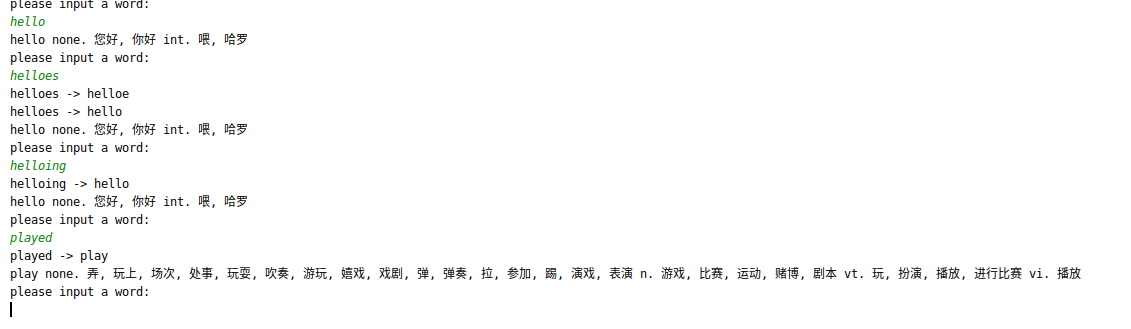
\includegraphics[scale=0.5]{imgs/test.png}    %添加图片,图片文件名为xiantu.jpg
	\caption{如图所示,算法能够对单词进行形态还原\label{fig:形态还原展示}}  %在图片下面的文字说明
\end{figure}


\newpage

\section{单词分词算法}
\subsection{作业要求}
Proj. 2 实现一个基于词典与规则的汉语自动分词系统。
(词典:http://nlp.nju.edu.cn/MT\_Lecture/dic\_ce.rar)


\subsection{实现思路}
通过正向最大匹配或者逆向最大匹配结合词典实现分词算法。

正向最大匹配相关代码:
\begin{lstlisting}[language=python]
def FMM(dict, text, max_len=5):
	"""
	正向最大匹配
	:param dict:
	:param text:
	:param max_len:单个词语的最大长度
	:return:
	"""
	rs = []
	start_pos = 0
	while start_pos < len(text):
		sub_word = text[start_pos:start_pos + max_len]
	while len(sub_word) > 0:
		if sub_word in dict or len(sub_word) == 1:
			rs.append(sub_word)
			start_pos += len(sub_word)
			break
		else:
			sub_word = sub_word[:-1]
	return rs
\end{lstlisting}


逆向最大匹配相关代码:
\begin{lstlisting}[language=python]
def RMM(dict, text, max_len=5):
	"""
	逆向最大匹配
	:param dict:
	:param text:
	:param max_len:单个词语的最大长度
	:return:
	"""
	rs = []
	start_pos = len(text)
	while start_pos > 0:
		split_start = max(start_pos - max_len, 0)
		split_end = start_pos
		sub_word = text[split_start:split_end]
		while len(sub_word) > 0:
			if sub_word in dict or len(sub_word) == 1:
				rs.append(sub_word)
				start_pos -= len(sub_word)
				break
			else:
				sub_word = sub_word[1:]
	rs.reverse()
	return rs

\end{lstlisting}

\subsection{结果展示}
\subsection{结果展示}
程序运行结果如下图所示:
\begin{figure}[!ht]\centering   %添加图片环境的配置
	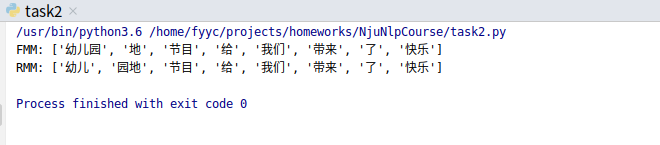
\includegraphics[scale=0.5]{imgs/wordSplit.png}    %添加图片,图片文件名为xiantu.jpg
	\caption{如图所示,使用正向匹配和逆向匹配算法对句子进行了分词\label{fig:句子分词展示}}  %在图片下面的文字说明
\end{figure}
\section{总结}  
深度学习并不是人工智能的全部,传统机器学习的知识也很重要。

\end{document}  %结束写文章
